\documentclass{article}
\usepackage[utf8]{inputenc}
\usepackage[T1]{fontenc}

\begin{document}
\usepackage{graphicx}

\textbf{ Tree for Personalized Web Documents Organization}
  
 \begin{center}
 
  
  Robert Moro, Maria Bielikova, Roman Burger 
 
 Slovak University of Technology in Bratislava

 Faculty of Informatics and Information Technologies
 
  Ilkovičova 2, 842 16 Bratislava, Slovakia 
  
  name.surname@stuba.sk
  \end{center}
  
 \textbf{Abstract.} Vast amount information and resources in the digital libraries and in general on the Web demands effective methods of archiving and organization. However, most of the existing solutions support only very specific use case scenarios, or are not flexible enough to accommodate to the changes in the document collections over time. We propose a method for web documents organization based on a facet view of the personal information structure. Facet chaining in a tree can create any depth of the structure and thus specify any context of resources. We enhanced this method by clustering similar resources and by using a special Search facet that allows users to specify arbitrary keyword queries as an input for collection’s categorization. In order to evaluate the proposed approach, we carried out a user study in the bookmarking system Annota .
 

 
 \textbf {Keywords:} digital library, personal information management, facet tree, web document clustering, user study, empirical evaluation, Annota 
 
 \section {Introduction}
 
 When browsing the Web, we encounter daily tens or even hundreds of web pages. For the purpose of their later retrieval and reference we bookmark those that are of any value, using either browser built-in bookmarking capability, or any of the available services, such as Delicious1, Readability2 or Pocket3. 


Similarly, with the continual shift of traditional libraries to the digital ones, we have now whole libraries within the reach of our hands (and mouse clicks). The researchers have to work with many resources when e.g. writing a thesis or a new paper; therefore, it becomes very important to them to be able to properly archive, maintain and retrieve all this information. 

Based on [14], we can identify three basic operations as a part of the (personal information) organization process: 
 
 \begin{description}
 
 \item[-]archiving a new resource – it is a process of expanding personal collection with new resources. Input to this process is the resource itself and metadata describing it, giving it context. It is up to the user how specific the context is. Output of the process is a resource archived in the user’s document collection.
 \item[-] retrieving an archived resource – it is a process of searching and retrieving the resource. Retrieving can be either destructive (resource is removed from the collection) or preserving (resource is kept in the collection). Resource query is the input to the process. Output is usually a set of best matching resources to the query.
 \item[-]editing an archived resource – it is a process of updating resource information, usually the metadata and relationships between resources. This process can be actually carried out as a series of destructive retrieval and archiving with new information
 \end{description}
 
The interface for personal documents organization and management should support all these operations minimizing the time and effort that the users have to spend in the process. Another important aspect to consider is, how the interface supports refactoring (restructuring) of the collection. 

In addition, the user needs may vary greatly between individuals, which is a fact often overlooked and ignored by typical frameworks and solutions for organizational tasks. Even users in the same domain can have radically different information management strategies as observed in [4]. These strategies are mostly based on personal preferences of individuals, but can also be influenced by various tasks or events (such as preparing a paper for the upcoming conference). 

In this paper, we explore the problem of personal information management of the web resources. We propose a new method of organizing and archiving web resources in an effective, easy to use and user friendly manner based on a concept of facet trees. We provide an empirical evaluation of the proposed method; we carried out a qualitative user study comparing the facet tree organization with folders commonly employed in many tools for personal documents management, such as Mendeley4. 
\section{related work}

There has been an extensive research in identifying main strategies commonly used in personal information management, based on which we can identify three basic strategies (or roles) that most users can be mapped to [3]: 

\begin{description}
\item [1.]piling strategy,
\item[2.]filing strategy
\item[3.]structuring strategy
\end{description}
Pilling strategy is on the context-free side of the organizational spectrum with the users archiving the resources in an unstructured pile (or a stack), while structuring strategy is on the context-full side. Filing strategy is somewhere in the middle.

 However,it is not about using average amount of context to describe resources, but it is rather more of a combination. Some parts of the personal library are in context-free zone, having stacks or piles of resources that user wants to dig in later (or never). Other parts of the library are reasonably structured, giving the user option to file new resources that are in great importance to the user.
 
  Typical task with personal libraries is recollecting and re-finding the archived or previously visited resources [1]. Semantic maps were used for this purpose in [13] in the domain of web search history. However, two of the most prevalent approaches of organizing web resources are bookmarks and tags services. Bookmarks usually utilize folder structure so they are suited for structuring strategy. Problem with maintaining huge structured libraries was tried to be solved using information retrieval algorithms such as clustering and classification. Authors in [5] used n-grams in documents to find clusters of similar documents. In [10] authors used incremental clustering to simulate more typical user scenarios. Hierarchical clustering based on the documents’ metadata and zoom-based navigation in the personal document collections have been utilized also in [9]. 
  
  Tags are keywords assigned to a web resource that have special meaning to the user and are usually visualized by a means of a tag cloud [11, 6]. The resource can be easily retrieved by the keyword-resource association. Tags represent one type of (in this case user-added) metadata. However, there can be other domain-specific metadata types.  Approach that uses them to navigate, search and explore the document collection is called faceted classification or search [8]. Facet browsers have been very successful in recent years; the extensive survey can be found in [18]. There are several problems associated, e.g. how to personalize the faceted interface to the user needs [15, 16]. 
  
  We have identified several limitations of the existing approaches: 
  
\begin{description}
\item[-]  low adaptability and limited support of multiple organization strategies – existing approaches usually support only one strategy for which they were designed, thus ignoring different personal organizational preferences of the users as well as their habits
\item[-] manual filing of a new resource – every resource has to be filed into a predefined structure manually, either into a folder or by assigning a tag. In addition, resources can be often assigned into only one category (folder). This is not true for tags, but on the other hand, they do not offer stable transparent library structure required for users using structuring strategy.
\item[-]limited support for reorganization of the collection – as the collection grows, the originally designed organizational structure can become too limited or simply no longer sufficient for maintaining the desired level of transparency and navigability. Existing approaches require manual reorganization which can be very demanding with respect to time and effort. 
\item[-] limited support for resources cleaning – it is common for filing strategy, however users usually need to manually edit each unsorted resource and file it into the right location in the library
\end{description}
Facets can address many of these limitations with their ability to automatically classify the collections of resources and to construct ad-hoc views. But because of their dynamic nature, they are rarely used for organization, in which the users usually rely on static personal structures, the state of which does not change until explicitly updated, thus allowing them to re-find the documents in the collection.
\section{Method for Personalized Web Resources Organization }
We propose our organization method based on the faceted search paradigm. The main advantage of faceted search is, that it allows users to construct arbitrary views on the underlying collection of documents, in our case the user’s personal resources library. 

Each resource in the collection is described by its associated metadata. In the domain of digital libraries of research papers, these would be e.g. authors, title, publication year, publication name, pages, etc. They represent non-overlapping (orthogonal) categories, i.e. facets, each describing particular aspect of a resource. Since they do not overlap, it is possible to combine them to better specify the given resource. 

 In order to find a balance between a static organization structure and a dynamic nature of facets, we utilize a concept of a facet tree based on the facet folders originally proposed in [17], which we enrich by the special Search facet and by the clustering of the documents with co-occurring facet values. 

\subsection{Facet Tree}
Facet tree allows the users to define hierarchies of the selected facets, thus automatically organizing their collection of documents. An example of such a hierarchy can be seen in Fig. 1; the user selected Keywords facet representing the keywords added to the documents by their authors at the first (root) level and Year facet representing the publication year at the second level. 

\begin{figure}
\centering
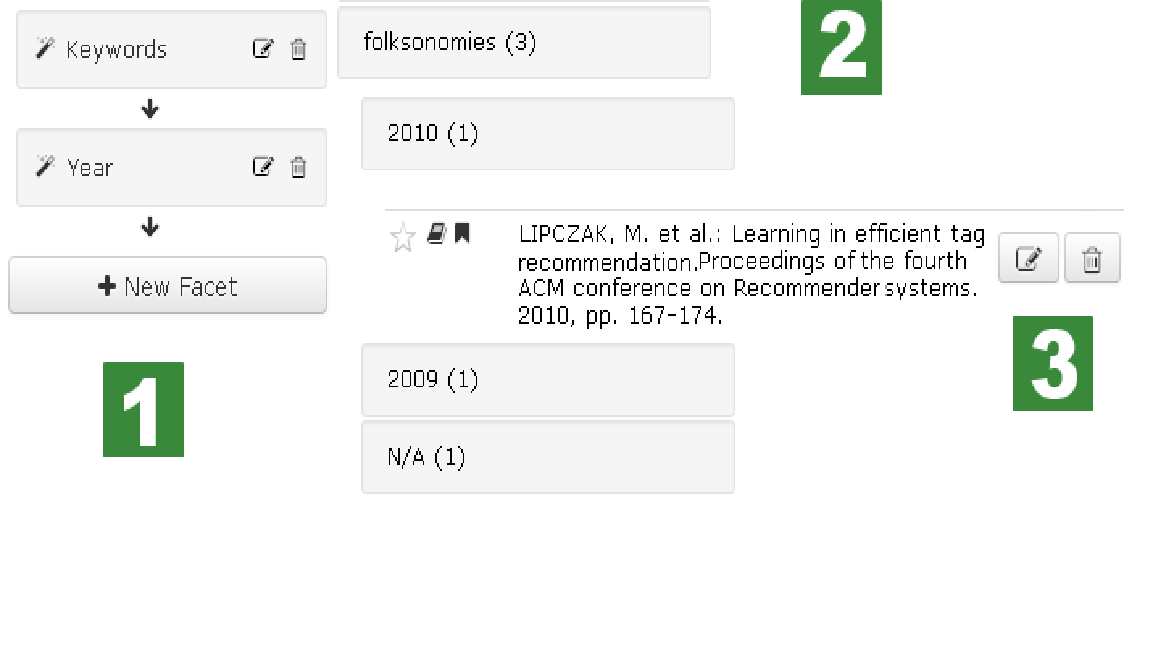
\includegraphics [width=\textwidth]{images/1.png}
\caption{Example of a facet tree hierarchy, with Keywords and Year facets selected (1). Folder with keyword folksonomies (2) is expanded showing three subfolders containing also NA value. User can edit the resource and its metadata or remove it from the collection 
\end{figure}

Thus, the collection is automatically divided into dynamic folders, where each folder represents one facet value (one author-specified keyword in our example, such as collaborative tagging). Each first-level folder is further divided into folders based on the publication year. Only non-empty folders are visualized to the users. In case of a missing facet’s value, the document is assigned into the special NA (not available) folder at its corresponding level. If the new document is added into collection, it will now be automatically added into existing structure based on its metadata. If the document matches more than one facet value (e.g. when it has more than one associated keyword), it will be added into each of the corresponding facet tree branches. This eliminates the problem the users often face when using the classical folders, which allow the documents to be added only at one place in the folder hierarchy. 

\begin{figure}
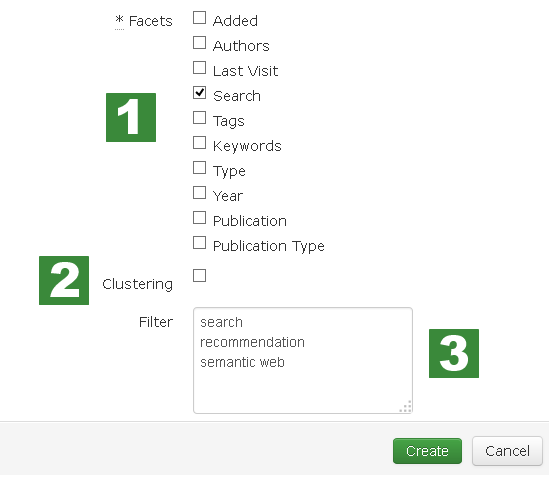
\includegraphics{image/obr.png}
\end{figure}

Important is, that the facet tree maintains its state (structure defined by the user). On the other hand, it can be easily adjusted if necessary. Individual facets in chained facet tree can be removed or added creating context views on demand (thus allowing to be used as a search tool as well). 

\subsection{Proposed Facets}

Because we focus on the domain of digital libraries and specifically on the collections of research papers, we use metadata usually associated with these documents as our facets, namely author, publication year, publication name and publication type (proceedings, journal, book etc.). We also use date when the document was added to the personal library and the date, when it was last accessed by the user.

 These types of metadata are more categorical and less descriptive, i.e. they do not convey much information regarding the papers’ content. For this purpose, we use already mentioned Keywords facet (representing the keywords specified by the papers’ authors). It is an example of a narrow folksonomy; however, as shown in [2] a broad folksonomy, i.e. created collaboratively by the users, is better for navigational purposes, as it provides more paths to the resources and utilizes directly the vocabulary of the users. Therefore, we use Tags facet as well. Faceted search and tag navigation are often viewed as two different approaches, but in their ability to construct arbitrary views of the information space the tags can be considered a special facet – the fact that we utilize in our proposed method.
 
  Since both the Keywords and Tags facet rely on the presence of associated metadata, they cannot handle the documents which have no keywords or tags associated (which is often the case especially with tags). Therefore, we propose a special Search facet, which allows the user to specify arbitrary keyword queries (see Fig. 2) using the filtering feature. It runs the specified queries in the search engine and shows the retrieved documents in the corresponding dynamic folders. Now every time a new document matching one of the queries is added, it will be retrieved in its folder.
  
   The filter can be used not only with the Search facet, but with other facets as well; in that case only matching facet values (and their corresponding folders) will be retrieved (e.g. when the user is interested only in certain authors or only in papers from certain year range). 
   \subsection{Identification of the Clusters of Related Documents }
   Keywords as well as Tags facets are useful for decomposing the collection by documents’ topics, but they can lead to many relatively small folders, when only a few documents share the same keyword or tag. Therefore, we provide the users with a possibility to cluster related documents with the co-occurring metadata values. This can be used with other facets as well, namely with Authors facet; in that case the authors are clustered based on the co-authorship relationships. 
   
    The clustering algorithm works as follows:
    
   It is a simple algorithm that merges two folders (based on their facet’s value), if they have at least half of the documents in common. Any given folder can be merged multiple times, thus allowing to find different clusters (cluster combinations) in the collection. In addition, it is possible that two folders with no intersection will end up together in a cluster, if there is a third folder with large enough intersection with both of them. This feature can prove to be useful, when considering e.g. the authors; we can find this way communities that have a common author, but are themselves different (not collaborating). 
  
  Other clustering algorithms could be used as well, e.g. k-means with k set based on the collections’ size and the desired average number of documents in a cluster, or hierarchical clustering algorithm that would allow to optimize also the number of the clusters presented to the user.
  
   Overall, clustering provides a better view of the collection and helps the users to discover hidden, or not so obvious relationship between the documents. Its power lies in further combination of facets. An interesting example would be to have Keywords facet at the first level, which clusters topically similar documents and then Authors facet on the second, which helps to visualize different communities working on the same research topics.
   
   \subsection{Support of Organization Strategies}
   
   Comparison of some of the features of the proposed facet tree organization method with the folders and tags organization paradigms can be seen in Table 1. Although tags allow resources to be in more than one category (by assigning more tags), it does not (usually) support hierarchy, only the relationships based on tags co-occurrence. As to the arbitrary views construction, it can be partially achieved also with folders, but it will always be a static structure, i.e. no ad-hoc views will be possible. Lastly, folders as well as tags require user action in order to categorize resource (inserting it to the selected folder or assigning tags). 
   
   
   \begin{table}
   \centering
   \caption{Feature comparison of the facet tree with most common organization paradigms.}
   \label{odkaz}
   \begin{tabular}{cccc }
   Resource in more categories &  Supports hierarchy & Provides
Arbitrary and ad-hoc views & Categorize resource
automatically \\
   
   \end{tabular}
   \end{table}
   
   
In addition, we have designed our approach to meet most of the common user needs and use cases in personal information management (PIM) strategies. Table 2 shows, how each of the user actions identified in [3] is mapped to the actions of our proposed method and reflects, how the result can be achieved using our proposed method.
   
    Archiving a new resource is simple, because it is done automatically based on the resource’s metadata. If the metadata is missing, the resource is added to the special NA folder. Users are thus motivated to clean their collection by adding the missing values as it directly influences the filing of the resource in the facet tree structure. Resources can be searched by either navigating in the facet tree structure or by creating an ad-hoc structure using the Search facet with the search query as its filter value.Lastly, the structure can be easily reorganized by changing the defined facet hierarchy
  
\section{Evaluation}
We evaluated our proposed approach in a bookmarking system Annota5 [12], which is being developed at our university as a part of a research project TraDiCe [7]. It allows users to bookmark any resource on the Web using the browser extension and manage their personal libraries using the web interface. Currently, it is used by 185 users, mostly consisting of the students and staff of our faculty.

 Annota provides special support for resources from digital libraries; it can automatically download the associated metadata, such as authors, title, year, etc. Users can annotate resources in their library with various annotation types (tags, comments or highlights). Important feature is sharing of the bookmarks within groups, thus supporting collaboration of researchers, or of students and their supervisors.
 
  Because Annota supports different kinds of personal resources management, namely folders and tags, we used it to compare our proposed approach with these traditional paradigms
  
 \subsection{Analysis of Folders Usage }
 We wanted to find out, how the users usually work with their document collections, how many documents these collections typically contain, or if users use folders to organize them. Therefore, we analyzed real usage data from Mendeley for 31 users who synchronized their libraries with Annota (mainly master or doctoral students).
 
  We summarize the data in the Table 3. We found out that the analyzed users have in average 233 documents in their personal libraries. This number is, however, influenced by a small number of users with more than 1000 documents. Average user has typically a lot less, with median being 95 documents per collection. 
 
 From the analyzed users 77.  uses folders to organize their documents, while 22.6 of the users have no folders. When they do have folders, they have typically no more than four and only at first level with no subfolders. Interestingly, even users, who use folders, have a quite large part of their collection unorganized with about 30 of documents, which do not belong to any folder. Only 19 of users have every document filed in an appropriate folder. This can suggest problems with folders’ usage; they can either not know, where they should file the document or simply do not have time to do it. Our data also show us that the ideal number of documents in a folder for the users is about 11, although there are some extremes as well .
 
 Based on these data, we can conclude that about 20 of users use piling strategy, while probably relying heavily on the provided search, 20 of users use structuring strategy and the largest group – about 60 – prefer filing strategy. There is also a difference in the folders’ purpose (based on the names of folders); 56 of users use folders predominantly for task-oriented organization, 24 organizes documents into folders based on their topics and 20 mixes both strategies  . 
 
 \subsection{User Study}
 In order to evaluate our proposed approach, we carried out a qualitative experiment – a user study with six participants. The participant were all male between 23 and 30 years with strong background in computer science and informatics (one master student, two doctoral students and three post-docs). 
 
 Our hypothesis was that the users can more easily (as measured by time and effort) manage their personal library using the facet tree as compared to the traditional folder approach. We also assumed that the facet tree structure will be robust enough to support various tasks without the need to change it.        
 
 
 \textbf{Participants of the Study.} Before the experiment we interviewed the participants to assess their information management habits and preferred strategies; results are summarized in Table 4. All the participants except one had previous experience with using Annota, although only two were using it actively to bookmark resources on the Web and in the digital libraries. Mendeley was stated as the preferred personal library management tool in five cases. One participant claimed not to use any available tool; instead, he uses folders provided by the operational system. 
 
 Five participants use folders, but their use is different. Only one participant prefers structuring strategy; two participants use folders based on their tasks (such as thesis, research paper etc.), two combine topic and task folders and one uses solely topic folders. One user claimed not use folders; he piles all the resources and uses search to retrieve the documents. Interestingly, the users tend not to change their defined structure; mostly because it suits their needs or because it would be too demanding.
 
 We can say that the distribution of preferences and strategies in the selected group of participants corresponds with the distribution discovered during the analysis of the folders usage described in previous section
 
 
\textbf{Experimental Setting.}
  Each participant was supposed to solve four tasks during the experiment. First task was to organize the given document collection using the folders  and facet tree (half of the participants used first folders and half facet tree). We considered the task to be successful, if the users identified the underlying topics in the dataset and organized it accordingly. 
  
   The second task was to archive a new source in the digital library, file it into folder structure constructed in the first task and try to locate the resource in the facet tree structure. Third task emulated conditions, when the users want to locate the resource they know they have in the library, but their information is incomplete (they do not remember all the necessary information); in our case we provided them the name of the first author, main topic and the conference, at which it was published. And lastly, the fourth task was to reorganize the collection using folders as well as facet tree.
   
    All the participants were provided with the same collection of 125 documents that was created as a subset of the Annota library dataset, which is also publicly available6 for research purposes. Overall, the dataset consists of approximately 16,000 documents which were collected as the users of Annota travelled in the information space of digital libraries, such as ACM DL7 or IEEE Xplore8. It thus contains groups of related documents which reflect research interests of the users. Beside the documents themselves, it contains extracted information on other entities, such as authors (currently 230,000) or author-added keywords (about 130,000). 
    
     The collection provided to the participants covered different topics, namely search, recommendation, tags and folksonomies, semantics, web and summarization with some random documents to simulate “noise”. 
     
     After each task, participants were asked to fill in the corresponding questions in the prepared questionnaire. Similarly, at the end of the experiment, we asked them to globally evaluate the proposed facet tree interface.
   
\textbf{Task 1.} The participants were confronted with a new interface. At first, they had problems with understanding the facets’ meaning, but after a quick explanation and a few trials with different facets, they were able to use it. For the organization of the collection, they almost exclusively used Keywords or Search facet at the first level. Typical sequence was to try the Keywords facet with clustering option first; this helped them to discover the underlying topics in the collection. For better results, they then proceeded to use the Search facet, where they could specify their own search terms.

 A few participants suggested that they would want to use combination of the Tags, Keywords and Search facets, as they are all concerned with the documents’ topics. At the second level (if they used it at all), participants used Authors or Year facet. Added and Last access facets were also mentioned as helpful, but they would prefer it as a sorting criterion instead of the separate facets.
 
  When the participants used first the facet tree, it helped them to quickly design the folder structure (more than a half of the participants agreed that it helped them with the domain overview). Otherwise the participants went through the documents in a sequence and created the corresponding folders. On the other hand, when creating the folders first, it also helped them to more quickly understand the collection; in that case, the participants usually applied directly the Search facet with the terms discovered during the folders creation. The chart in the Fig. 3 shows, how the users perceived the effort when creating the organizational structure, which is in favor of the facet tree . 
  


We also enquired about the satisfaction with the resulting structure (see Fig. 4). On the scale 1 to 5, the four was the most frequent with the facet tree. Folders were rated variously, but on average worse. As a main disadvantage of folders was perceived the possibility of assigning the resource only to a single folder in the hierarchy. 

\textbf{Task 2.}Finding the newly archived resource and filing it into appropriate folder was trivial, because it was first on the list (resource were sorted by the date of last access). However, two participants reported, that they hesitated, into which folder to file the resource. 

Locating the resource in the facet tree was for most of the participants easy as well. The metadata from the added resource were extracted correctly and thus the participants did not have to locate it in the NA folder. However, they appreciated that the facet tree approach motivates them to clean the data (i.e. to add missing metadata values) in order to remove the resources from the NA folder to the appropriate one. 

One participant had a Keyword facet at the first level, which resulted into going over all the clusters, which was not the most effective way and was therefore reported as very time-consuming. When he changed the structure to a better one, he found it immediately. Other participants changed their structures as well; it was an example of an ad-hoc query.

  At this point, many participants suggested that they would not like to change the structure for each task; they would like to have more facet trees for repeating tasks, i.e. structures with more facets at the same level, which would provide them different views over the same collection. 

\textbf{Task 2.} Re-finding a resource in a collection is a very frequent task. We often remember only a partial information, e.g. only author, or part of the title etc. This can be problematic to do with folders, because they usually provide only one view of the collection. In addition, if the users hesitate between two folders when archiving the resource and then decide for one of them, they will probably check both of them in the future, because they will not remember, where they filed it; a problem reported by one of our participants. Also, if we forget to file the resource (as is the case in 30 of the users’ documents according to our analysis), the structure becomes useless and the user has to go over the resources sequentially or use a search. 

Re-finding with facet tree depends on the used structure and the available metadata. If the current structure does not allow for easy location of the resource, users can easily change it; this happened in 67 of cases during our experiment . 

\textbf{Task 4.}  We also discussed with the participants the task of reorganizing their personal libraries. According to our pre-experimental questionnaire, this does not seem a very frequent task. The participants tend to add new folders to their library, but do not change the existing ones. One of the reasons is probably the effort that it requires – 60 of participants rated merging as well as partitioning of the folders as difficult (rating 4 and 5 on the 5-point scale). It largely depends on the provided folder interface, but it usually means going over the whole collection manually and moving the resources or folders to the new ones, which can be very time consuming. 

Here, the facet tree clearly prevails, as was proved in the three experimental tasks. Cost of changing the tree is very low, allowing the users to experiment and use it also to explore new views of the collection or create an arbitrary ad-hoc view for the task at hand.    

\section{Discussion and Conclusions}
In this paper, we proposed a facet tree approach as a method for organization of Web resources with a special focus on the digital libraries. Our main contribution is in providing the clustering of the facets’ values in order to create more meaningful grouping of documents and the special Search facet which enables to organize documents based on user-specified search queries. 

We evaluated our proposed approach in bookmarking system Annota by carrying out a user study. Our results indicate that the facet tree is an efficient tool for organization of the personal libraries of the web resources:

\begin{itemize}
\item[-]It provides users with an overview of the domain and helps them to uncover not so obvious or even hidden relationships using a combination of facets and clustering of the related documents based on their facet’ values.
\item[-]It supports creation of stable organizational structures, as well as arbitrary ad-hoc queries (views) for the task at hand
\item[-]It automatically files the resources into a predefined structure
\item[-]It can help retrieve documents with only a partial information about it
\item[-]It supports various personal information management strategies (piling, filing and structuring) and different folder usage styles (topic-based, task-oriented). Taskoriented folders can be easily achieved with an added effort of tagging the resources according to the task and then using the Tags facet.
\end{itemize}}

As to our hypothesis, we proved that the facet tree outperforms the folders approach in terms of time and effort when organizing the collection for the first time or in the process of its reorganization as well as when locating (re-finding) the resource in the collection. It is also easier to add new resources to the structure, since this happens automatically.  

On the other hand, our second hypothesis that the structure will be robust to changes proved to be false. As it turned out, most of the participants reorganized structure for each task. As a solution, we propose the concept of facet forest of individual trees that provides different views at the collection at the same time and thus eliminates the need to create a new facet tree structure again and again for the repeating tasks.

 We can conclude that the participants of our user study appreciated the clustering option and used it frequently with the Keywords facet. On the other hand, there were too many small clusters (of one or two documents) that could have been clustered together, as the ideal number of first level clusters seems 7±2 with 10-15 documents in each cluster according to our analysis. If there are more documents, than this structure could contain, the second level should be added following the same rule of thumb. For most of the users collections the second level would be enough, since it could contain 7x7x10 =  490 documents and as we found out, users have typically far less documents than that (with median of 95).

 In addition, the participants found the Search facet very useful, as it allowed them to formulate their own search queries and organize resources accordingly. This gives them a powerful tool, especially if it is further combined with Keywords and Tags facet as was suggested by numerous participants during the experimental evaluation.
 
 The reaction and feedback of the participants was overall positive. The average rating of the global satisfaction with the interface at its current state was 3.3 (on the fivepoint scale). 
 
  Positive is that the participants did not feel constrained by the fact that they could not directly change the filing of the resource within the automatically generated clusters. In fact, they spoke against it, saying, that then they could easily forget, that they did such changes and it would make it harder to re-find the resources in the future. On the other hand, hiding the unwanted resources from the search facet that match the queries would be appreciated by some of the participants.
 
  Most of the participants (5 out of 6) were content with the provided functionality and would give even higher global rating if their suggestions to the functionality would be incorporated. From these the most important that we plan to add to the next version of the interface are the following: 
  
\begin{description}
\item[-] Enable to create more independent facet trees (i.e. a facet forest) in order to provide different views at the collection at once and to lower the need to create new views for each new task, i.e. to make the structure more stable with respect to the future changes.
\item[-]Combine Tags, Keywords and Search facet into one Topic facet. Also enable to assign names to specified facet values, which can be more or less complicated user queries. Because we log search queries performed by the users in the digital libraries, we could extend this functionality to actually suggest the users the queries for the combined Topic facet based on their search history. 
\item[-]Add the possibility to set granularity of the clustering algorithm and avoid creating too small clusters (or too big for that matter). 
\item[-] Enable sorting of the resources in the dynamic folders based on the document metadata values, as well as their easier filtering. 
\item[-] Add examples of facets or previews to make them easier to understand and use by the novice users. 
\end{description}

In addition, there is a potential to use the proposed approach not only for the organization of the personal document collections. Other viable scenarios include exploratory search or finding of new resources in the public library that match the criteria given by the facet tree structure.
 

\textbf{Acknowledgement } This work was partially supported by the Scientific Grant Agency of the Slovak Republic, grant No. VG1/0675/11 and VG1/0971/11 and by the Slovak Research and Development Agency under the contract No. APVV-0208-10.






\section{Introduction}

\end{document}
